\documentclass{article}

\usepackage[margin=1in]{geometry} 
\usepackage{amsmath,amsthm,amssymb,amsfonts, fancyhdr, color, comment, graphicx, environ,bbm}
\usepackage[dvipsnames]{xcolor}
\usepackage{subcaption}
\usepackage{mdframed}
\usepackage[shortlabels]{enumitem}
\usepackage{indentfirst}
\usepackage{hyperref}
\usepackage{placeins}
\usepackage{comment} %Comment large blocks
\usepackage{xfrac}
\usepackage{float} % To use "H" to force tables to be where wanted
\usepackage{booktabs} % Makes output from knittr:kable look better
\usepackage{parskip} %No indents for paragraphs
\usepackage[shortlabels]{enumitem} % To enumerate with letters
\hypersetup{
 colorlinks=true,
 linkcolor=blue,
 filecolor=magenta, 
 urlcolor=blue,
}
\pagestyle{fancy}
\usepackage{todonotes}

\newcommand{\E}{\mathbb{E}}
\renewcommand{\H}{\mathcal{H}}
\renewcommand{\L}{\mathcal{L}}
\newcommand{\dU}[1]{\ensuremath\frac{\partial u}{\partial #1}}
\newcommand{\dV}[1]{\ensuremath\frac{\partial v}{\partial #1}}
\newcommand{\ppx}[2]{\ensuremath\frac{\partial #1}{\partial #2}}
\newcommand{\ddx}[2]{\ensuremath\frac{d #1}{d #2}}
\newcommand{\indp}{\perp\!\!\!\perp} 

%\usepackage{mathpazo} %Dylan's fancy math bullshit that I don't want
\usepackage{microtype}
\usepackage{graphicx}
\usepackage{setspace}

%Footnote without a number
\newcommand\blfootnote[1]{%
  \renewcommand\thefootnote{}\footnote{#1}%
  \addtocounter{footnote}{-1}%
}

% Problem formatting [Alex]

\newenvironment{problem}[1]
    { \begin{mdframed}[backgroundcolor=Periwinkle!20] \textbf{(#1)} }
    {  \end{mdframed}}
% Define solution environment
\newenvironment{solution}{\textbf{Solution}\\}
%%%%%%%%%%%%%%%%%%%%%%%%%%%%%%%%%%%%%%%%%%%%%
%Fill in the appropriate information below
\lhead{Problem Set 1}
\rhead{Empirical Analysis} 
\title{Problem Set 3}
\author{Alex Weinberg \and Isaac Norwich \and Jose M. Quintero}

%%%%%%%%%%%%%%%%%%%%%%%%%%%%%%%%%%%%%%%%%%%%%
\begin{document}
\maketitle

Our code can be found in this GitHub respository: \url{https://github.com/jmquintero925/Metrics-III/tree/main/ps3}

%Q1 - Alex
%Q2 - Isaac
%Q3 - Jose
%Q4 - Isaac


%%%%%%%%%%%%%%%%%%%%%%%%%%%%%%%%%% QUESTION 1 %%%%%%%%%%%%%%%%%%%%%%%%%%%%%%%%%
\section*{Problem 1}
Suppose you want to understand how neighborhoods affect children's
future earnings. You collect an i.i.d. sample $\left\{ Y_{i},D_{i}\right\} _{i=1}^{n}$,
where $Y_{i}$ is a child's income in adulthood and $D_{i}$ indicates
whether that child grows up in a low-poverty neighborhood $(1=yes$
, $0=no)$. 

% ------------------------------------
\begin{problem}{a}
Define the ATE, ATT, and ATUT in this setting. When can you estimate
them via OLS? Do you believe that these restrictions you impose are
likely to hold? Briefly explain. 
\end{problem}

Yes, I define them as follows
\begin{align*}
ATE & :=E\left[Y_{1}-Y_{0}\right]\\
ATT & :=E\left[Y_{1}-Y_{0}|D=1\right]\\
ATU & :=E\left[Y_{1}-Y_{0}|D=0\right]
\end{align*}

These are hard to estimate using OLS because OLS is going to pick
up on selection bias. I decompose the OLS estimand for with respect
to the ATT but the idea is the same for ATU, ATE, etc. 
\begin{align*}
\beta^{OLS} & =\frac{Cov\left[Y,D\right]}{Var\left[D\right]}\\
 & =E\left[Y_{1}|D=1\right]-E\left[Y_{0}|D=0\right]\\
 & =\underbrace{E\left[Y_{1}|D=1\right]-E\left[Y_{0}|D=1\right]}_{ATT}+\underbrace{E\left[Y_{0}|D=1\right]-E\left[Y_{0}|D=0\right]}_{selection}
\end{align*}

However if $D\perp Y_{1},Y_{0}$ then we have treatment randomly assigned
so then $E\left[Y_{0}|D=1\right]-E\left[Y_{0}|D=0\right]=0$ and we
are good. OLS recovers $ATE=ATT=ATU$.

\rule[0.5ex]{1\columnwidth}{1pt}

% ------------------------------------
\begin{problem}{b}
Suppose you collect data about $X_{i}$, the parents' annual incomes
when the child is young. 
\end{problem}


(i) Under selection-on-observables (i.e. $Y_{d,i}\perp D_{i}\mid X_{i}$
), explain how to estimate the ATE. 

\rule[0.5ex]{1\columnwidth}{1pt}

If I assume that $Y_{d,i}\perp D_{i}\mid X_{i}$ then I define the
ATE and use the independence assumption to get
\begin{align*}
ATE & :=E\left[E\left[Y_{1}|X\right]-E\left[Y_{0}|X\right]\right]\\
 & =E\left[E\left[Y_{1}|D=1,X\right]-E\left[Y_{0}|D=0,X\right]\right]
\end{align*}

(ii) Do you believe selection-on-observables is likely to hold in
this case? Briefly explain. 

\rule[0.5ex]{1\columnwidth}{1pt}

Selection on observables seems hard to justify here. The assumption
requires tht 
\[
E\left[Y_{d}|D=0,X\right]=E\left[Y_{d}|D=1,X\right]\qquad\forall d,X
\]

In words, in our context, that says \emph{conditional on parental
income, children in poor neighborhoods would have had the same outcomes
as children who grew up in rich neighborhoods. }I further assume that
there is enough support (i.e. we observe rich families in poor neighborhoods). 
\begin{itemize}
\item This assumption fails because I believe parental income is an outcome
variable. If one of the mechanisms by which bad neighborhoods hurt
kids is by reducing parental income (e.g by poor access to jobs) then
we are controlling for a mechanism - not kosher.
\item This fails also because there is unobserved selection bias in the
parents who choose to live in different neighborhoods. 
\begin{itemize}
\item Consider poor parents who choose to live in rich neighborhoods because
they are very excited about the good schools available for their children
there. Those parents are likely also taking other steps to improve
their childs outcomes. So when we compare means we end up incorporating
selection bias (here parental quality). 
\end{itemize}
\end{itemize}

\begin{problem}{c}
Suppose there exists a program
that gives housing vouchers to underserved families with young children.
Each voucher subsidizes the cost of moving to a low-poverty neighborhood.
These vouchers are randomly assigned to families, and not everyone
who is offered a voucher accepts one. Let $Z_{i}$ indicate whether
a child's family receives a voucher $(1=yes,0=no)$. Assume that your
population consists of children whose families are eligible for vouchers. 
\end{problem}


(i) Define the compliers, always-takers, never-takers, and defiers
in this setting. 

\rule[0.5ex]{1\columnwidth}{1pt}

\begin{align*}
D_{1}=1, & D_{0}=0\tag{compliers}\\
D_{1}=0, & D_{0}=1\tag{defiers}\\
D_{1}=1, & D_{0}=1\tag{always takers}\\
D_{1}=0, & D_{0}=0\tag{never takers}
\end{align*}

In this setting Always-Takers move to rich neighborhoods regardless
of voucher. Never-takers similarly never move, regardless of voucher.
Compliers move if they get the voucher and don't move otherwise. Defiers
move if they don't get the voucher and don't move if they do. 

(ii) Argue whether $Z_{i}$ is a valid instrument for $D_{i}$. 

\rule[0.5ex]{1\columnwidth}{1pt}

We need four conditions to have a valid instrument. 
\begin{enumerate}
\item \textbf{Random assignment.} Satisfied here because voucher given by
lottery.
\[
Y_{d,z},D_{z}\perp Z
\]
\item \textbf{Exclusion.} I believe that winning the voucher lottery only
affects childrens outcomes via the treatment. I believe this because
the voucher size is likely small and does not create income effects.
\[
Y_{d,1}=Y_{d,0}\qquad\forall d
\]
\item \textbf{First stage.} This is testable. It seems likely the voucher
would have an effect on movement decisions if voucher size large enough.
\[
E\left[D_{1}-D_{0}\right]\neq0
\]
\item \textbf{Monotonicity (Uniformity)}. This seems sensible. I can't imagine
that people who receive a voucher are less likely to move. 
\[
D_{1}-D_{0}\geq0
\]
\end{enumerate}
\rule[0.5ex]{1\columnwidth}{1pt}

(iii) In general, the ATT and LATE
are not the same, since the ATT is a weighted average of two effects:
one on always-takers and one on compliers. Show that this is the case. 

\rule[0.5ex]{1\columnwidth}{1pt}

Recall the definition of the ATT. Use the law of total probability.

\begin{align*}
ATT & :=E\left[Y_{1}-Y_{0}|D=1\right]\\
 & =E\left[Y_{1}-Y_{0}|D_{1}>D_{0},D=1\right]Pr\left(D_{1}>D_{0}\right)+E\left[Y_{1}-Y_{0}|D_{1}=D_{0},D=1\right]Pr\left(D_{1}>D_{0}\right)\\
\end{align*}

We can see that the ATT is the weighted average of the treatment effect
for two groups. The first group $D_{1}>D_{0}$ are the compliers.
The second group $D_{1}=D_{0}=1$ are the always-takers. Note that
$D_{1}\geq D_{0}$ by the monotonicity assumption. 

\rule[0.5ex]{1\columnwidth}{1pt}

(iv) Assuming $Z_{i}$ is a valid
instrument for $D_{i}$, will running IV estimate the ATE? If so,
explain. If not, specify the exact conditions under which the LATE
equals the ATE. 

\rule[0.5ex]{1\columnwidth}{1pt}

No, IV will not estimate the ATE. It will estimate the LATE. We showed
this in class. If the entire population are compliers then 
\[
ATE=LATE
\]

I will do the decomposition to show this is true. 

If the $LATE_{always}=LATE_{complier}=LATE_{never}$ then LATE is
also ATE.

(v) Describe how to consistently estimate the average treatment effect
of $Z_{i}$ on $Y_{i}$.

\rule[0.5ex]{1\columnwidth}{1pt}

I want to estimate 
\[
ATE_{Z}=E\left[Y|Z=1\right]-E\left[Y|Z=0\right]
\]

Recall
\begin{align*}
Y & =Y_{1}D+Y_{0}\left(1-D\right)\\
D & =D_{1}Z+D_{0}\left(1-Z\right)
\end{align*}

Since $Z$ is randomly assigned we can run OLS. 
\begin{align*}
\beta^{OLS,Z} & =\frac{Cov\left[Y,Z\right]}{Var\left[Z\right]}\\
 & =\frac{E\left[YZ\right]-E\left[Y\right]E\left[Z\right]}{E\left[Z^{2}\right]-E\left[Z\right]^{2}}\\
 & =\frac{E\left[Y|Z=1\right]-E\left[Y|Z=0\right]}{E\left[D|Z=1\right]-E\left[D|Z=0\right]}
\end{align*}

I can write the denominator as
\begin{align*}
E\left[D|Z=1\right]-E\left[D|Z=0\right] & =E\left[D_{1}|Z=1\right]-E\left[D_{0}|Z=0\right]\\
 & =E\left[D_{1}-D_{0}\right]\tag{random assignment}\\
 & =E\left[D_{1}-D_{0}|D_{1}>D_{0}\right]Pr\left(D_{1}>D_{0}\right) \\
 &+E\left[D_{1}-D_{0}|D_{1}=D_{0}\right]Pr\left(D_{1}=D_{0}\right)+E\left[D_{1}-D_{0}|D_{1}<D_{0}\right]Pr\left(D_{1}<D_{0}\right)\\
 & =E\left[D_{1}-D_{0}|D_{1}>D_{0}\right]Pr\left(D_{1}>D_{0}\right)\\
 & =Pr\left(D_{1}>D_{0}\right)
\end{align*}

where the always-takers, never-takers drop out because $D_{1}-D_{0}=0$
and defiers are ruled out by assumption $Pr\left(D_{1}<D_{0}\right)=0$.

The numerator becomes
\begin{align*}
E\left[Y|Z=1\right]-E\left[Y|Z=0\right] & =E\left[Y_{1}D+Y_{0}\left(1-D\right)|Z=1\right]-E\left[Y_{1}D+Y_{0}\left(1-D\right)|Z=0\right]\\
 & =E\left[Y_{1}\left(D_{1}Z+D_{0}\left(1-Z\right)\right)+Y_{0}\left(1-\left(D_{1}Z+D_{0}\left(1-Z\right)\right)\right)|Z=1\right] \\
 & -E\left[Y_{1}\left(D_{1}Z+D_{0}\left(1-Z\right)\right)+Y_{0}\left(1-\left(D_{1}Z+D_{0}\left(1-Z\right)\right)\right)|Z=0\right]\\
 & =E\left[Y_{1}\left(D_{1}Z\right)+Y_{0}\left(1-\left(D_{1}Z\right)\right)|Z=1\right]-E\left[Y_{1}\left(D_{0}\left(1-Z\right)\right)+Y_{0}\left(1-\left(D_{0}\left(1-Z\right)\right)\right)|Z=0\right]\\
 & =E\left[Y_{1}D_{1}+Y_{0}\left(1-D_{1}\right)|Z=1\right]-E\left[Y_{1}D_{0}+Y_{0}\left(1-D_{0}\right)|Z=0\right]\\
 & =E\left[Y_{1}D_{1}+Y_{0}\left(1-D_{1}\right)-Y_{1}D_{0}+Y_{0}\left(1-D_{0}\right)\right]\tag{random assignment}\\
 & =E\left[Y_{1}\left(D_{1}-D_{0}\right)-Y_{0}\left(D_{1}-D_{0}\right)\right]\\
 & =E\left[\left(Y_{1}-Y_{0}\right)\left(D_{1}-D_{0}\right)\right]\\
 & =E\left[\left(Y_{1}-Y_{0}\right)|\text{complier}\right]Pr\left(D_{1}>D_{0}\right)+0\times Pr\left(D_{1}=D_{0}\right)+E\left[\left(Y_{1}-Y_{0}\right)\right]Pr\left(D_{1}<D_{0}\right)\\
 & =E\left[\left(Y_{1}-Y_{0}\right)|\text{complier}\right]Pr\left(D_{1}>D_{0}\right)
\end{align*}

where for the last inequality always takers, never takers, and defiers
drop out. 

Divide numerator by denominator to get 
\begin{align*}
\beta^{IV} & =\frac{E\left[Y|Z=1\right]-E\left[Y|Z=0\right]}{E\left[D|Z=1\right]-E\left[D|Z=0\right]}\\
 & =\frac{E\left[\left(Y_{1}-Y_{0}\right)|\text{complier}\right]Pr\left(D_{1}>D_{0}\right)}{Pr\left(D_{1}>D_{0}\right)}\\
 & =E\left[\left(Y_{1}-Y_{0}\right)|\text{complier}\right]
\end{align*}


\newpage
%%%%%%%%%%%%%%%%%%%%%%%%%%%%%%%%%% QUESTION 2 %%%%%%%%%%%%%%%%%%%%%%%%%%%%%%%%%
\section*{Problem 2}
Consider the following model of supply and demand:
\begin{align*}
\begin{array}{cl}
Q^{D}=\beta_{0}^{D}-\beta_{1}^{D} P+U^{D} & \text{(Demand)} \\
Q^{S}=\beta_{0}^{S}+\beta_{1}^{S} P+U^{S} & (\text{Supply})
\end{array}
\end{align*}
Throughout this exercise, assume that $E\left(U^{D}\right)=E\left(U^{S}\right)=E\left(U^{D} U^{S}\right)=0$, and suppose you observe the market in equilibrium (i.e. $Q^{D}=Q^{S}$ ). Your goal is to estimate $\beta_{1}^{D}$ and $\beta_{1}^{S}$.

\begin{problem}{a}
Show that $P$ is endogenous in both equations.
\end{problem}
\begin{solution}
To show that $P$ is endogenous, we want to show that the covariance of $P$ and each error term, $U^D$ and $U^S$ is not zero. First, since we know $Q^S=Q^D$, we can plug in and solve for $P$ as such:
\begin{align*}
    Q^S &= Q^D \\
    \beta_{0}^{S}+\beta_{1}^{S} P+U^{S} &= \beta_{0}^{D}-\beta_{1}^{D} P+U^{D}\\
    \implies P &= \frac{\beta_{0}^{D} - \beta_{0}^{S} + U^D - U^S}{\beta_1^S+\beta_1^D}
\end{align*}

So now we can plug the above in for $P$ when we look at the covariance of $P$ and the error terms:
\begin{align*}
    \operatorname{Cov}(P,U^D) &= \operatorname{Cov}\left(\frac{\beta_{0}^{D} - \beta_{0}^{S} + U^D - U^S}{\beta_1^S+\beta_1^D}, U^D \right) \\
    &= \operatorname{Cov}\left(\frac{\beta_{0}^{D} - \beta_{0}^{S}}{\beta_1^S+\beta_1^D}, U^D \right) + \operatorname{Cov}\left( \frac{U^D - U^S}{\beta_1^S+\beta_1^D}, U^D \right) \\
    &= \frac{1}{\beta_1^S+\beta_1^D} \left( \operatorname{Var}\left(U^D, U^D \right) - \operatorname{Cov}\left(U^S, U^D \right) \right) \\
    &= \frac{1}{\beta_1^S+\beta_1^D} \left( E[U^D U^D] - E[U^S U^D] \right) \neq 0
\end{align*}
which we know is not equal to zero since the variance of $U^D$ is $E[U^D U^D]>0$ and the covariance of the two errors is $E[U^S U^D]\geq0$.

Similarly, for the supply equation, just replace all the superscript $D$'s with $S$'s and the same relationship holds. This is obvious ince $P$ contains $U^S$ and $U^D$ so will be endogenous both equations.
\end{solution}

\begin{problem}{b}
Suppose you observe a variable $Z$ that affects only the supply, so that:
\begin{align*}
\begin{aligned}
&Q^{D}=\beta_{0}^{D}-\beta_{1}^{D} P+U^{D} \\
&Q^{S}=\beta_{0}^{S}+\beta_{1}^{S} P+\kappa Z+U^{S}
\end{aligned}
\end{align*}
Assume that $E\left(Z U^{D}\right)=E\left(Z U^{S}\right)=0$ and $\kappa \neq 0$. Show that $Z$ satisfies both instrument exogeneity and instrument relevance. Do these properties hold if $Z$ also affects demand?
\end{problem}
\begin{solution}
\underline{Instrument Exogeneity} requires that $U^D \perp Z$. We are told to assume that $E[Z U^D]=0$, thus by assumption instrument exogeneity holds.

\underline{Instrument Relevance} requires that $Cov(P,Z)\neq0$. To show this, let's first solve for $P$ in terms of the RHS coefficients and variables like we did in part A. 
\begin{align*}
    Q^S &= Q^D \\
    \beta_{0}^{S}+\beta_{1}^{S} P + \kappa Z +U^{S} &= \beta_{0}^{D}-\beta_{1}^{D} P+U^{D}\\
    \implies P &= \frac{\beta_{0}^{D} - \beta_{0}^{S} - \kappa Z + U^D - U^S}{\beta_1^S+\beta_1^D}
\end{align*}
Now plug in to the covariance:
\begin{align*}
    \operatorname{Cov}(Z,P) &= \operatorname{Cov} \left(Z,\frac{\beta_{0}^{D} - \beta_{0}^{S} - \kappa Z + U^D - U^S}{\beta_1^S+\beta_1^D} \right) \\
    &= \frac{1}{\beta_1^S+\beta_1^D} \left( -\kappa \operatorname{Var} \left(Z \right) + \operatorname{Cov} \left(Z, U^D - U^S \right) \right) \\
    &= \frac{-\kappa}{\beta_1^S+\beta_1^D} \operatorname{Var} \left(Z \right)
\end{align*}
Therefore, given $\kappa\neq 0$, we have that the covariance between $Z$ and $P$ is not 0 and thus instrument relevance is satisfied..

These properties do not hold if $Z$ also affects demand. If this is the case, we are back in the world of Part A, where we have a simultaneity problem.
\end{solution}

\begin{problem}{c}
Using the setup from $(b)$, express both $P$ and $Q$ as linear functions of $Z$. Then, assuming that $Z$ is a valid instrument, show how to consistently estimate $\beta_{1}^{D}$ from data $\left\{Q_{i}, P_{i}, Z_{i}\right\}_{i=1}^{n}$.
\end{problem}
\begin{solution}
We can re-write our equation for $P$ from above to more clearly delineate how it is a linear function of $Z$:
\begin{align*}
    P 
    %&= \underbrace{\frac{\beta_{0}^{D} - \beta_{0}^{S}}{\beta_1^S+\beta_1^D}}_{\equiv \pi_0} + \underbrace{\frac{-\kappa}{\beta_1^S+\beta_1^D}}_{\equiv \pi_1} Z + \underbrace{\frac{U^D - U^S}{\beta_1^S+\beta_1^D}}_{\equiv \varepsilon}
    &= \frac{\beta_{0}^{D} - \beta_{0}^{S}}{\beta_1^S+\beta_1^D} +  \frac{-\kappa}{\beta_1^S+\beta_1^D} Z + \frac{U^D - U^S}{\beta_1^S+\beta_1^D}
\end{align*}
Plugging this result in for $P$ in the equation for $Q^D$ gives:
\begin{align*}
    Q^D &= \beta_{0}^{D}-\beta_{1}^{D} P+U^{D} \\
    &= \beta_{0}^{D}-\beta_{1}^{D} \left(\frac{\beta_{0}^{D} - \beta_{0}^{S}}{\beta_1^S+\beta_1^D} + \frac{-\kappa}{\beta_1^S+\beta_1^D} Z + \frac{U^D - U^S}{\beta_1^S+\beta_1^D} \right) +U^{D} \\
    &= \beta_{0}^{D}-\beta_{1}^{D} \frac{\beta_{0}^{D} - \beta_{0}^{S}}{\beta_1^S+\beta_1^D} 
        + \beta_1^D \frac{\kappa}{\beta_1^S+\beta_1^D} Z 
        - \beta_1^D \frac{U^D - U^S}{\beta_1^S+\beta_1^D} + U^{D} \\
\end{align*}
To consistently estimate $\beta_1^D$ from data $\{Q_i,P_i,Z_i\}_{i=1}^n$, we can use the IV estimator:
\begin{align*}
    \beta_1^{D,IV} &= - \left(\frac{1}{n-1} \sum_{i=1}^{n} (Z_i-\bar{Z}) (P_i-\bar{P}) \right)^{-1}\left(\frac{1}{n-1} \sum_{i=1}^{n} (Z_{i}-\bar{Z})(Q_{i}-\bar{Q}) \right)
\end{align*}
Note: we add the negative since we are really estimating is $-\beta_1^D$.

Since we are just-identified, this is equivalent to running the 2SLS procedure where we consistently estimate the coefficient on $Z$ in a regression of $Q^D$ on $Z$ and scale it by the coefficient of $Z$ in the the first stage regression of $P$ on $Z$.
\end{solution}

\begin{problem}{d}
Now, suppose that consumers in the market face a tax ``$\tau$'', so that:
\begin{align*}
\begin{aligned}
    &Q^{D}=\beta_{0}^{D}-\beta_{1}^{D}(P+\tau)+U^{D} \\
    &Q^{S}=\beta_{0}^{S}+\beta_{1}^{S} P+U^{S}
\end{aligned}
\end{align*}
Assume $\tau \perp\left(U^{D}, U^{S}\right)$. Given $\left\{Q_{i}, P_{i}, \tau_{i}\right\}$, show how to consistently estimate $\beta_{1}^{D}$ and $\beta_{1}^{S}$. Give an economic interpretation to the coefficients $\beta_{1}^{D}$ and $\beta_{1}^{S}$. Justify your responses.
\end{problem}
\begin{solution}
In parts B and C, we worked with an exogenous supply shifter. Now, we have a tax $\tau$ that acts as an exogenous ($\tau \perp (U^D, U^S)$) demand shifter. To consistently estimate $\beta_1^S$, we follow similar steps to above.

First, let's solve for $P$ in terms of $\tau$ and $\beta$s:
\begin{align*}
    Q^{S} &= Q^{D}  \\
    \beta_{0}^{S}+\beta_{1}^{S} P+U^{S} &= \beta_{0}^{D}-\beta_{1}^{D}P-\beta_{1}^{D}\tau+U^{D}\\
    P &= \frac{\beta_0^D-\beta_0^S}{\beta_{1}^{S} + \beta_{1}^{D}} 
       - \frac{\beta_1^D}{\beta_{1}^{S} + \beta_{1}^{D}} \tau 
        + \frac{U^D-U^S}{\beta_{1}^{S} + \beta_{1}^{D}} 
\end{align*}
Plugging in for $P$ in the supply equation gives:
\begin{align*}
    Q^{S} &= \beta_0^S + \beta_1^S \frac{\beta_0^D-\beta_0^S}{\beta_{1}^{S} + \beta_{1}^{D}}
        - \beta_1^S \frac{\beta_1^D}{\beta_{1}^{S} + \beta_{1}^{D}} \tau
        + \beta_1^S \frac{U^D-U^S}{\beta_{1}^{S} + \beta_{1}^{D}}  + U^S
\end{align*}
We can now estimate this reduced form regression ($Q^S=Q$ on $\tau$) to obtain the coefficient on $\tau$, which gives us:
\begin{align*}
    \left( \frac{1}{n-1} \sum_{i=1}^n (\tau_i-\bar{\tau})^2  \right)^{-1}\left( \frac{1}{n-1} \sum_{i=1}^n (\tau_i-\bar{\tau})( Q_i - \bar{Q}) \right)  \to
    -\beta_1^S \frac{\beta_1^D}{\beta_{1}^{S} + \beta_{1}^{D}} \tag{$Q$ on $\tau$}
\end{align*}
If we then run the first stage regression of $P$ on $\tau$ to obtain an estimate of the coefficient multiplying $\tau$, we get:
\begin{align*}
   \left( \frac{1}{n-1} \sum_{i=1}^n (\tau_i-\bar{\tau})^2  \right)^{-1} \left(\frac{1}{n-1} \sum_{i=1}^n (\tau_i-\bar{\tau}) ( P_i - \bar{P}) \right)  \to - \frac{\beta_1^D}{\beta_{1}^{S} + \beta_{1}^{D}} \tag{$P$ on $\tau$}
\end{align*}
Dividing the first by the second is the IV estimator for $\beta_1^S$ of:
\begin{align*}
    \beta_1^{S,IV} &= \left(\frac{1}{n-1} \sum_{i=1}^{n-1} (\tau_i-\bar{\tau}) (P_i-\bar{P}) \right)^{-1}\left(\frac{1}{n-1} \sum_{i=1}^{n-1} (\tau_{i}-\bar{\tau})( Y_{i}  - \bar{Y}) \right)
\end{align*}

To consistently estimate $\beta_1^D$, we can take our equation for $P$ from above and add $\tau$ to both sides to obtain:
\begin{align*}
    P + \tau &= \frac{\beta_0^D-\beta_0^S}{\beta_{1}^{S} + \beta_{1}^{D}} 
      + \frac{\beta_1^S}{\beta_{1}^{S} + \beta_{1}^{D}} \tau 
      + \frac{U^D-U^S}{\beta_{1}^{S} + \beta_{1}^{D}}
\end{align*}
We can consistently estimate this equation because $\tau \perp (U^D,U^S)$. When we do, we obtain:
\begin{align*}
    \left( \frac{1}{n-1} \sum_{i=1}^n (\tau_i-\bar{\tau})^2 \right)^{-1} \left( \frac{1}{n-1} \sum_{i=1}^n (\tau_i-\bar{\tau}) (P_i+\tau_i-\bar{P}-\bar{\tau})  \right) \to \frac{\beta_1^S}{\beta_{1}^{S} + \beta_{1}^{D}} \tag{$P+\tau$ on $\tau$}
\end{align*}
Diving our estimate from the reduced form regression of $Q$ on $\tau$ by the above result yields a consistent estimate of $-\beta_1^D$. This is essentially the IV estimate from a reduced form of $Q$ on $\tau$ scaled by the first stage of $P+\tau$ on $\tau$.

Assuming that observed prices, quantities, and taxes are in log form, what we get are the price elasticities of demand ($\beta_1^D$) and supply ($\beta_1^S$). The price elasticity of demand is the percent decrease in quantity demanded when $P+\tau$ increases by 1\%. Similarly, the price elasticity of demand is the percent increase in quantity supplied when $P$ goes up.

%%%%%%%%%% COMMENT BLOCK
\begin{comment}
Now plugging this in to the equation for $Q^D$ gives:
\begin{align*}
    Q^{D} &= \beta_{0}^{D}-\beta_{1}^{D}(P+\tau)+U^{D}\\
    &=\beta_{0}^{D}
    -\beta_{1}^{D}\frac{\beta_0^D-\beta_0^S}{\beta_{1}^{S} + \beta_{1}^{D}}
    -\beta_{1}^{D}\frac{\beta_1^S}{\beta_{1}^{S} + \beta_{1}^{D}} \tau 
    -\beta_{1}^{D}\frac{U^D-U^S}{\beta_{1}^{S} + \beta_{1}^{D}} 
    + U^D
\end{align*}
So we can consistently estimate the coefficients from this regression, since :

\todo[inline]{The summation part on the LHS looks exactly the same as a part above, which would mean that $\beta_1^S=\beta_1^D$???}
Then dividing this estimate by the estimate from the first stage regression of $P$ on $\tau$, which gave us $-\frac{\beta_1^D}{\beta_1^S+\beta_1^D}$, would give us just $\beta_1^D$.
\end{comment}
\end{solution}

\begin{problem}{e}
Now, suppose that $\left(\beta_{1}^{D}, \beta_{1}^{S}\right)$ are unobserved random variables and that $\left(\beta_{0}^{D}, \beta_{0}^{S}\right)$ are constants. Return to the setup from (b), assuming that $Z \perp \beta$ and $\kappa$ is constant. Write down the IV estimand in terms of $\left(\beta_{1}^{D}, \beta_{1}^{S}\right)$. When does running IV consistently estimate $E\left(\beta_{1}^{D}\right)$ ?
\end{problem}
\begin{solution}
For this problem, I believe we also need to assume joint independence of the $\beta$s and $U$s in order to write down the IV estimand in terms of $\beta$s that are unobserved random variables. That is, we need to also assume A3 on top of the given A1 and A2: 
\begin{align}
    (U^S,U^D) \perp Z \tag{A1} \\
    (\beta_1^D,\beta_1^S) \perp Z \tag{A2} \\
    (\beta_1^D,\beta_1^S,U^S,U^D) \perp Z \tag{A3}
\end{align}

Let's recall our equation for $P$ from part B:
\begin{align*}
    P &= \frac{\beta_{0}^{D} - \beta_{0}^{S}}{\beta_1^S+\beta_1^D} + \frac{ - \kappa}{\beta_1^S+\beta_1^D} Z + \frac{U^D - U^S}{\beta_1^S+\beta_1^D}    
\end{align*}
And recall the IV estimand is:
\begin{align*}
    -\beta_1^{D,IV} &= \frac{\operatorname{Cov}(Z,Q^D)}{\operatorname{Cov}(Z,P)}
\end{align*}
Let's first break out the numerator:
\begin{align*}
    \operatorname{Cov}(Z,Q^D) &= \operatorname{Cov}\left(Z, \beta_{0}^{D}-\beta_{1}^{D} P+U^{D}  \right) \tag{Plug in for $Q^D$} \\ 
    &= \operatorname{Cov}\left(Z, \beta_{0}^{D}-\beta_{1}^{D} \frac{\beta_{0}^{D} - \beta_{0}^{S}}{\beta_1^S+\beta_1^D} + \beta_1^D \frac{\kappa}{\beta_1^S+\beta_1^D} Z - \beta_1^D \frac{U^D - U^S}{\beta_1^S+\beta_1^D} + U^{D}  \right) \tag{Plug in for $P$} \\
    &= \operatorname{Cov}\left(Z, -\beta_{1}^{D} \frac{\beta_{0}^{D} - \beta_{0}^{S}}{\beta_1^S+\beta_1^D} \right) + \operatorname{Cov}\left(Z,\beta_1^D \frac{\kappa}{\beta_1^S+\beta_1^D} Z \right) - \operatorname{Cov}\left(Z, \beta_1^D \frac{U^D - U^S}{\beta_1^S+\beta_1^D} - U^{D}  \right) \\
    &= (\beta_{0}^{S} - \beta_{0}^{D})\underbrace{\operatorname{Cov}\left(Z,  \frac{\beta_{1}^{D}}{\beta_1^S+\beta_1^D} \right)}_\text{$=0$ from A2} + \kappa \operatorname{Cov}\left(Z, \frac{\beta_1^D}{\beta_1^S+\beta_1^D} Z \right) - \underbrace{\operatorname{Cov}\left(Z, \beta_1^D \frac{U^D - U^S}{\beta_1^S+\beta_1^D} - U^{D}  \right)}_\text{$=0$ from A3} \\
    &=  \kappa \operatorname{Cov}\left(Z, \frac{\beta_1^D}{\beta_1^S+\beta_1^D} Z \right) \\
    &=  \kappa E\left [ \frac{\beta_1^D}{\beta_1^S+\beta_1^D} \right] \operatorname{Var}(Z)  \tag{From A2}
\end{align*}

Now the denominator:
\begin{align*}
    \operatorname{Cov}(Z,P) &= \operatorname{Cov} \left(Z,\frac{\beta_{0}^{D} - \beta_{0}^{S}}{\beta_1^S+\beta_1^D} + \frac{ - \kappa}{\beta_1^S+\beta_1^D} Z + \frac{U^D - U^S}{\beta_1^S+\beta_1^D}  \right) \tag{Plug in for P}\\
    &= \underbrace{\operatorname{Cov} \left(Z,\frac{\beta_{0}^{D} - \beta_{0}^{S}}{\beta_1^S+\beta_1^D} \right)}_\text{$=0$ from A2} +  \operatorname{Cov} \left(Z, \frac{ - \kappa}{\beta_1^S+\beta_1^D} Z \right) + \underbrace{\operatorname{Cov} \left(Z, \frac{U^D - U^S}{\beta_1^S+\beta_1^D}  \right)}_\text{$=0$ from A3} \\
    &= -\kappa \operatorname{Cov} \left(Z, \frac{Z}{\beta_1^S+\beta_1^D} \right) \\
    &= -\kappa E\left[ \frac{1}{\beta_1^S+\beta_1^D}\right] \operatorname{Var} \left(Z  \right) \tag{From A3}
\end{align*}
\end{solution}
So combining these two results gives:
\begin{align*}
    -\beta_1^{D,IV} &= \frac{\operatorname{Cov}(Z,Q^D)}{\operatorname{Cov}(Z,P)}  \\
    &= - \frac{E\left [ \frac{\beta_1^D}{\beta_1^S+\beta_1^D} \right]}{E\left[ \frac{1}{\beta_1^S+\beta_1^D}\right]}
\end{align*}
So only if we assume that $\beta_1^D \perp (\beta_1^S+\beta_1^D)$ can we consistently estimate $\beta_1^D$, since the above becomes $\beta_1^{D,IV}=E[\beta_1^D]$.

\begin{problem}{f}
If $\beta_{1}^{D}, \beta_{1}^{S} \geq 0$ and $\beta_{1}^{S}$ is constant, how does the IV estimand from (e) compare with $E\left(\beta_{1}^{D}\right)$ ? Discuss the policy relevance of the IV estimator under heterogeneous treatment effects.
\end{problem}
\begin{solution}
If $\beta_1^S$ is a constant, then we can simplify the numerator from the IV estimand from Part E as such:

\begin{align*}
    E\left [ \frac{\beta_1^D}{\beta_1^S+\beta_1^D} \right] &=  \frac{E[\beta_1^D]}{\beta_1^S+E[\beta_1^D]}
\end{align*}
And the denominator becomes:
\begin{align*}
    E\left[ \frac{1}{\beta_1^S+\beta_1^D}\right] &=  \frac{1}{\beta_1^S+E[\beta_1^D]}
\end{align*}
So combining gives:
\begin{align*}
    \beta_1^{D,IV} &= \frac{E\left [ \frac{\beta_1^D}{\beta_1^S+\beta_1^D} \right]}{E\left[ \frac{1}{\beta_1^S+\beta_1^D}\right]} \tag{Part E answer} \\
    &=\frac{\frac{E[\beta_1^D]}{\beta_1^S+E[\beta_1^D]}}{\frac{1}{\beta_1^S+E[\beta_1^D]}} \\
    &= E[\beta_1^D]
\end{align*}
\end{solution}
What this relationship says is that our IV estimand is the average of heterogeneous coefficients (LATEs). Normally, with heterogeneous treatment effects we think of the IV estimand as the average treatment effects on the compliers, however this result shows that we are not conditioning on any compliers. Why is that? Well first, let's think of this market in terms of there being one supplier and many buyers, where we only observe market equilibrium quantities, prices, and the supply shifter. Why only one supplier? Since $\beta_1^S$ is a constant and so too is $\kappa$, we only have one supplier or can think of there being many identical suppliers. With $\beta_1^D$ being a random variable, what we have is a distinct set of buyers whose aggregate quantity purchased at a given price is observed, but who each have their own $\beta_{1,i}^D$. 

Now that we know we have many buyers and one supplier, who are the compliers and why are we not conditioning on them? In this context, since our instrument is a supply shifter, the suppliers are those being impacted by the instrument. Since we only have one supplier and we know $\kappa\neq 0$, we know that when $Z$ changes by $\delta Z$, $Q^S$ must change by $\kappa \delta Z$. Thus the one supplier is always a complier and we do not need to worry about always-takers, never-takers, or defiers in this setting. We are simply using the supply shifter to trace out the heterogeneous demand curves for each buyer and then estimating a weighted average of each buyers' price elasticity in $E[\beta_1^D]$. In addition, since we assumed that $\beta_1^D \geq 0$, we know that all buyers respond to an the price change in the same direction.

\newpage
%%%%%%%%%%%%%%%%%%%%%%%%%%%%%%%%%% QUESTION 3 %%%%%%%%%%%%%%%%%%%%%%%%%%%%%%%%%
\section*{Problem 3}
Consider the adjusted set of assumptions conditional on covariates:
\begin{itemize}
    \item Exogeneity: $\left(Y_{0}, Y_{1}, D_{0}, D_{1}\right) \indp Z \mid X$
    \item Relevance: $P(D=1 \mid X, Z=1) \neq P(D=1 \mid X, Z=0)$ a.s.
    \item Monotonicity: $P\left(D_{1} \geq D_{0} \mid X\right)=1$ a.s.
    \item Overlap: $P(Z=1 \mid X) \in(0,1)$ a.s.
\end{itemize}

\begin{problem}{a}
Show that you can identify $\operatorname{LATE}(x)=E(Y_{1}-Y_{0} \mid \underbrace{T=c}_{\text {compliers }}, X=x)$.
\end{problem}
\begin{solution}
Consider the Wald estimate
\begin{equation*}
    \frac{\E\left[Y\vert Z=1\right]-\E\left[Y\vert Z=0,X\right]}{\E\left[D\vert Z=1,X\right]-\E\left[D\vert Z=0,X\right]}
\end{equation*} and lets show that this indeed identifies the ATE. To do so, begin by manipulating the numerator in the following way:
\begin{align*}
    \E\left[Y\vert Z=1,X\right]-\E\left[Y\vert Z=0,X\right] &= \E\left[Y_1D+Y_0(1-D)\vert Z=1,X\right]-\E\left[Y_1D+Y_0(1-D)\vert Z=0,X\right] \\ 
     &= \E\left[Y_1D_1+Y_0(1-D_1)\vert Z=1,X\right]-\E\left[Y_1D_0+Y_0(1-D_0)\vert Z=0,X\right] \\ 
     &= \E\left[Y_1D_1+Y_0(1-D_1)\vert X\right]-\E\left[Y_1D_0+Y_0(1-D_0)\vert X\right] \\
     &= \E\left[(Y_1-Y_0)(D_1-D_0) \vert X\right] \\
     &= \sum_{t\in\{a,n,c,d\}}\E\left[(Y_1-Y_0)(D_1-D_0) \vert T=t X\right]\Pr(T=t)
\end{align*}
were $a$ is the group of always takers, $n$ are the never takers, $c$ are the compliers and $d$ are defiers. Note that monotonicity assumption implies that the probability of defiers is 0. Additionally, $D_1-D_0=0$ if $t\in\{a,n\}$. Then, our past equation can be simplified to 
\begin{equation*}
    \E\left[Y\vert Z=1,X\right]-\E\left[Y\vert Z=0,X\right] = \E\left[(Y_1-Y_0) \vert T=c, X\right]\Pr(T=c)
\end{equation*}
where I am using the fact that $D_0,D_1\in\{0,1\}$ and thus for compliers $D_1-D_0=1$. For the denominator the process is very similar:
\begin{align*}
    \E\left[D\vert Z=1,X\right]-\E\left[D\vert Z=0,X\right] &= \E\left[D_1\vert Z=1,X\right]-\E\left[D_0\vert Z=0,X\right] \\ 
    &= \E\left[D_1\vert X\right]-\E\left[D_0\vert X\right] \\ 
    &= \E\left[D_1-D_0\vert X\right] \\
     &= \sum_{t\in\{a,n,c,d\}}\E\left[(D_1-D_0) \vert T=t X\right]\Pr(T=t) \\ 
     &= \Pr(T=c)
\end{align*}
Putting both pieces together the Wald estimate can be expressed as 
\begin{equation*}
    \frac{\E\left[Y\vert Z=1\right]-\E\left[Y\vert Z=0,X\right]}{\E\left[D\vert Z=1,X\right]-\E\left[D\vert Z=0,X\right]} =  \E\left[(Y_1-Y_0) \vert T=c, X\right]
\end{equation*}
\end{solution}

\begin{problem}{b}
Show $\E\left[Y_{1}-Y_{0} \mid T=c\right]=\E\left(\frac{\operatorname{LATE}(X) P(T=c \mid X)}{P(T=c)}\right)$.
\end{problem}
\begin{solution}
Begin by using the LIE to use the definition of LATE given in the question:
\begin{align*}
    \E\left[Y_{1}-Y_{0} \mid T=c\right] &= \E\left[\E[Y_1-Y_0\vert T=c, X]\vert T=c \right] \tag{LIE}\\ &= \E[\text{LATE}(X)\vert T=c] \tag{Def Late} \\
    &= \frac{\E[\text{LATE}(X)\mathbbm{1}\{T=c\}]}{\Pr(T=c)} \tag{CE} \\ 
    &= \frac{\E[\E[\text{LATE}(X)\mathbbm{1}\{T=c\}\vert X]]}{\Pr(T=c)} \\ 
    &= \frac{\E[\text{LATE}(X)\E[\mathbbm{1}\{T=c\}\vert X]]}{\Pr(T=c)} \\ 
    &=\frac{\E[\text{LATE}(X)\Pr(T=c\vert X)]}{\Pr(T=c)} \\ 
    &=\E\left[\frac{\text{LATE}(X)\Pr(T=c\vert X)}{\Pr(T=c)}\right]
\end{align*}
\end{solution}

\begin{problem}{c}
Suppose that $X$ is discrete (a set of binary indicators), that excluded instruments are $Z$ and $X Z$, where $Z \in\{0,1\}$, and that the model is fully saturated. Show that:
\begin{align*}
\beta_{T S L S}=E\left(\operatorname{LATE}(X) \frac{\operatorname{Var}(p(X, Z) \mid X)}{E(\operatorname{Var}(p(X, Z) \mid X))}\right)
\end{align*}
\end{problem}
\begin{solution}
Begin by noting that two stage least square estimator, using the Frisch-Waugh-Lovell theorem, is
\begin{equation*}
    \beta_{TSLS} = \frac{\cov(Y,\tilde{\hat{D}})}{\var(\tilde{\hat{D}})}
\end{equation*}
where $\hat{D}=\blp{D}{X,Z}$. Note that because the first stage is fully saturated and $D$ is a binary variable, then the best linear approximation approximates fully identifies $\E[D\vert X,Z]=\Pr(D=1\vert X,Z) = p(X,Z)$. Again, the Frisch-Waugh-Lovell theorem defines
\begin{align*}
    \tilde{\hat{D}} &= \hat{D} - \blp{\hat{D}}{X} \\ 
    &= \E[D\vert X,Z] - \E[\E[D\vert X,Z]\vert X] \\ 
    &= p(X,Z) - p(X)
\end{align*}
where the second equality uses the fact again that the regression is fully saturated on $X$ and thus identifies the conditional expectation. Putting this two facts together, the two stage estimator is 
\begin{align*}
    \beta_{TSLS} = \frac{\cov(Y,p(X,Z) - p(X))}{\var(p(X,Z) - p(X))}
\end{align*}
Observe that $\tilde{\hat{D}}$ is the residual of a linear regression and thus $\E[\tilde{\hat{D}}]=0$. Thus, the previos can be simplified even more:
\begin{equation*}
    \beta_{TSLS} = \frac{\E[Y(p(X,Z) - p(X)]}{\E[(p(X,Z) - p(X))^2]}
\end{equation*}
Next, note that since everything is within an expectation, I can arbitrarily take conditional expectations within by the LIE. In particular $\E[p(X)]=\E[\Pr(D=1\vert X)]=\E[\E[D\vert X]] = \E[D]$. Using this fact
\begin{align*}
    \E[(p(X,Z) - p(X))^2] &= \E[(p(X,Z) - p(X))(p(X,Z) - p(X))] \\ 
    &= \E[(D - \E[D\vert X])(p(X,Z) - \E[p(X,Z)\vert X])] \\ 
    &= \E[\cov(D,p(X,Z)\vert X)] \\ 
\end{align*}
Since $Z$ is a binary variable then $p(X,Z)=p(X,1)Z+p(Z,0)(1-Z)$. Using the bilinearity of the covariance we can rewrite it as 
\begin{align*}
    \E[(p(X,Z) - p(X))^2] &= \E[\cov(D,p(X,Z)\vert X)] \\ 
    &= \E[\cov(D,p(X,1)Z+p(Z,0)(1-Z)\vert X)] \\  
    &= \E[\cov(D,Z\vert X)p(X,1) + \cov(D,1-Z\vert X)p(X,0)] \\ 
    &= \E[\cov(D,Z\vert X)(p(X,1)-p(X,0))]
\end{align*}
A similar argument can be applied to the numerator
\begin{align*}
    \E[Y(p(X,Z) - p(X)] &= \E[Y(p(X,Z)-\E[p(X,Z)\vert X]] \\ 
    &= \E[\cov(Y,p(X,Z)\vert X)] \\ 
    &= \E[\cov(Y,Z\vert X)(p(X,1)-p(X,0))]
\end{align*}
From part (a) note that the Wald estimate can be written in terms of the covarinces. Specifically, 
\begin{equation*}
    \text{LATE}(X) = \frac{\cov(Y,Z\vert X)}{\cov(D,Z\vert X)}
\end{equation*}
Using this fact we can rewrite the two stage least square estimate as 
\begin{equation*}
    \beta_{TSLS} = \frac{\E[\text{LATE}(X)\cov(D,Z\vert X)]}{\E[\cov(D,Z\vert X)]}
\end{equation*}
To finish the proof we use the fact that 
\end{solution}

\begin{problem}{d}
Show that, for binary $D$ and $Z$, and for any function $G=g(Y, X, D)$ :
\begin{align*}
\E[G \mid T=c]=\frac{1}{P(T=c)} \E(\kappa G), \quad \text { where: } \kappa=1-\frac{D(1-Z)}{P(Z=0 \mid X)}-\frac{Z(1-D)}{P(Z=1 \mid X)}
\end{align*}
\end{problem}
\begin{solution}
Begin by noting that 
\begin{equation*}
    D(1-Z) = \begin{cases}
    1 &\mbox{if } D_0 = 1 \\ 
    0 &\mbox{otherwise}
    \end{cases}
\end{equation*}
and similarly 
\begin{equation*}
    (1-D)Z = \begin{cases}
    1 &\mbox{if } D_1 = 0 \\ 
    0 &\mbox{otherwise}
    \end{cases}
\end{equation*}
Using these two facts note that 
\begin{equation*}
    \E[\kappa\vert T=t,Z,D,X,Y]= \begin{cases}
    1 &\mbox{if } t = c \\ 
    0 &\mbox{if } t\in\{a,n,d\}
    \end{cases}
\end{equation*}
Thus by using the law of total probability 
\begin{align*}
    \E[\kappa\vert Z,D,X,Y] &=\sum_{t\in\{a,n,c,d\}} \Pr(T=t)  \E[\kappa\vert T=t,Z,D,X] \\ 
    &= \Pr(T=c) \E[\kappa\vert T=c,Z,D,X] \\ 
    &= \Pr(T=c)
\end{align*}
With this in mind, is just a matter of using the definition of conditional expectation:
\begin{align*}
    \E[G\vert T=c] &= \frac{1}{\Pr(T=c)} \E[G\mathbbm{1}\{T=c\}] \\ 
    &= \frac{1}{\Pr(T=c)} \E[\E[G\mathbbm{1}\{T=c\}\vert Z,D,X,Y]] \\ 
    &= \frac{1}{\Pr(T=c)}\E[G\E[\mathbbm{1}\{T=c\}\vert Z,D,X,Y]] \\ 
    &= \frac{1}{\Pr(T=c)}\E[G\Pr(T=c)] \\ 
     &= \frac{1}{\Pr(T=c)}\E[G \E[\kappa\vert Z,D,X,Y]] \\ 
      &= \frac{1}{\Pr(T=c)}\E[\E[G\kappa\vert Z,D,X,Y]] \\ 
      &= \frac{1}{\Pr(T=c)}\E[G\kappa] \\ 
\end{align*}
\end{solution}

\newpage
%%%%%%%%%%%%%%%%%%%%%%%%%%%%%%%%%% QUESTION 4 %%%%%%%%%%%%%%%%%%%%%%%%%%%%%%%%%
\section*{Problem 4}
Seats in Dutch medical schools are assigned through a lottery. Applicants to medical studies in the Netherlands are assigned to lottery categories based on their high school grades. The categories differ by the probability to be awarded a place (to win the lottery). If people lose a lottery they can try again the following year. Below you find a link to a dataset that has results from peoples' first lottery outcomes for participants in 1988 and 1989, and whether they attended medical school, as well as earnings from a survey that was sent out in 2007.

\begin{center}
    \url{https://www.dropbox.com/s/dy6cmnmmvvkfv4l/lottery dta?dl=1}    
\end{center}

You plan to estimate the return to attending medical school $(D)$ on earnings in 2007 $(\ln w)$ using the lottery outcome $(Z)$ as your instrument. Answer the following questions.

\begin{problem}{a}
Discuss instrument exogeneity, exclusion and monotonicity.
\end{problem}
\begin{solution}
\underline{Instrument exogeneity} is $(Y_0,Y_1,D_0,D_1) \perp Z$. Here, we have $\ln w$ instead of $Y_1$ and $Y_0$, but we can think of potential outcomes in terms of log wage for individuals who did and did not attend medical school. Recall that random assignment plus exclusion restriction equals instrument exogeneity. While we have random assignment, it is not random across individuals but rather within lottery categories, which are determined by high school grades. Thus we do not have instrument exogeneity.

\underline{Exclusion} is $Y_{d,1}=Y_{d,0}$. For this to hold, it would mean that the lottery does not impact future earnings other than through impacting whether or not people to go medical school. If winning the lottery induces individuals to exert more effort (due to greater returns to education, for instance), that effort may causally increase future earnings in a way that is independent of going to medical school, and thus we violate the exclusion restriction. 

However, if we think that individuals always exert maximum effort, another violation to the exclusion restriction is that we do not capture how many times each person has entered the lottery, so our measure of 2007 earnings could be the wrong outcome variable. Think of someone who loses a few lottery attempts, but sticks with it and finally gets accepted. They go to medical school, but when they are surveyed in 2007 their earnings are lower than if they had won on the first chance due to the delayed start to medical school. Hopefully the number of individuals who apply many times is none (or perhaps we can remove them from the sample).

\underline{Monotonicity} is $D_1 \geq D_0$ -- all those affected by the lottery are affected in the same direction. We could tell a story where someone being more likely to win the lottery makes them less likely to go to medical school due to outside options, but this seems implausible in a sample of individuals who have actively applied to medical school. Therefore, it seems plausible to make this assumption.

\end{solution}

\begin{problem}{b}
Assess instrument relevance.
\end{problem}
\begin{solution}
\underline{Instrument relevance} is $E[D_{1,i}-D_{0,i}]\neq 0$ or equivalently $\pi_1 \neq 0$ in $D = \pi_0 + \pi_1 Z + \varepsilon$. Since this is a testable assumption, we will use the data provided to regress $D$ on $Z$ and test whether the coefficient on $Z$ is statistically indistinguishable from 0.

From the below table, we can conclude that the instrument is relevant since we get a t-statistic of 26.67, which means the coefficient is statistically indistinguishable from 0 at any reasonable level of confidence.
\begin{table}[H]
    \centering
    \begin{tabular}{l*{1}{c}}
\hline\hline
                    &\multicolumn{1}{c}{Attended medical school}\\
\hline
Admitted through the lottery&       0.520\\
                    &    (0.0195)\\
[1em]
Constant            &       0.410\\
                    &    (0.0162)\\
\hline
Observations        &        1476\\
\hline\hline
\multicolumn{2}{l}{\footnotesize Standard errors in parentheses}\\
\end{tabular}

    \caption{Testing Instrument Relevance}
\end{table}
\end{solution}

\begin{problem}{c}
Estimate the return to medical school on earnings in 2007 using IV. Interpret the results.
\end{problem}
\begin{solution}
To estimate the return to medical school on earnings in 2007 using IV, we run TSLS in Stata and report the results in the table below. I also ran TSLS ``manually'' by regressing $D$ on $Z$, then predicting $D$ using the regression to create $\widehat{D}$, and finally regressing $\ln w$ on $\widehat{D}$. Of course, the results are identical.

\begin{table}[H]
    \centering
    \begin{tabular}{l*{2}{c}}
\hline\hline
                    &\multicolumn{1}{c}{2SLS manually}&\multicolumn{1}{c}{2SLS using ivregress}\\
\hline
Attended medical school&       0.187&            \\
                    &    (0.0504)&            \\
[1em]
$\widehat{D}$ from D on Z&            &       0.187\\
                    &            &    (0.0505)\\
[1em]
Constant            &       3.011&       3.011\\
                    &    (0.0407)&    (0.0407)\\
\hline
Observations        &        1476&        1476\\
\hline\hline
\multicolumn{3}{l}{\footnotesize Standard errors in parentheses}\\
\end{tabular}

    \caption{Return to medical school on log earnings}
\end{table}

These results show us that attending medical school increases log wage in 2007 by 0.187, or rather increases wages in 2007 by $\exp(0.187)-1=20.6\%$. We would like to interpret this causally, but given the lack of instrument exogeneity and exclusion restriction, we cannot. As Professor Mogstad said, IV results with non-credible assumptions go into the special filing cabinet!
\end{solution}

\begin{problem}{d}
Count the number of compliers. Compare them to the population of applicants by gender.
\end{problem}
\begin{solution}
Let $C \in \{c,a,n \}$ denote which group an individual is in. Then we have:
\begin{align*}
    p_a &\equiv P(C=a) = P(C=a|Z=0) \\
    p_n &\equiv P(C=n) = P(C=n|Z=1) \\
    p_c &\equiv P(C=c) = 1 - p_a - p_n
\end{align*}
Equivalently, we know that compliers are those for which $D_{1,i}>D_{0,i}$, so the proportion of compliers in the sample is:
\begin{align*}
    P(D_{1,i}>D_{0,i}) &= E[D_{1,i}>D_{0,i}] \\
    &= E[D_1] - E[D_0] \\
    &= E[D|Z=1] - E[D|Z=0]
\end{align*}
Both of these we can estimate in the data and are reported in the table below. We see that the proportion of men that are compliers is higher than the proportion of women, even though the number of women that are compliers is higher. This raw count different is due to the fact that the sample is 64.2\% female, so there are just more women. The difference in the proportion of males and females that are compliers is something to think about in terms of conditioning on covariates.

\begin{table}[H]
    \centering
    \begin{tabular}{l*{2}{c}}
\hline\hline
            &        $\%$&           N\\
\hline
Female      &       0.504&     464.372\\
Male        &       0.546&     303.080\\
Total       &       0.520&     767.969\\
\hline\hline
\end{tabular}

    \caption{Estimated Complier Count}
\end{table}
\end{solution}

\begin{problem}{e}
Is the IV estimate an estimate of the ATT? Explain why or why not.
\end{problem}
\begin{solution}
The IV estimate is an estimate of the local average treatment effect (LATE), under the usual assumptions. Since the assumptions do not hold here, we have not actually estimated the LATE. Even still, the ATT only equals the LATE under our IV assumptions when $P(D_1>D_0)=0$ (this is partially shown in Question 1 Part Ciii). That is, no one who loses the lottery ($Z=0$) goes on to attend medical school ($D=1$).\footnote{For my own sake, this is not the same as saying there are no always-takers! There could be always takers who won the lottery, but would have still gone to medical school if they had lost it.}
\end{solution}

\begin{problem}{f}
Estimate the mean and distribution of $Y_{0}$ and $Y_{1}$ for compliers.
\end{problem}
\begin{solution}
To estimate the mean of $Y_0$ and $Y_1$ for compliers, I follow Slide 20 of week3.pdf to get:
\begin{align*}
    E[Y_0|C=c] &= \frac{ E[ Y \cdot (1-D) | Z=1] - E[Y \cdot (1-D) | Z=0] }{ E[1-D|Z=1]-E[1-D|Z=0] } \\
    E[Y_1|C=c] &= \frac{ E[ Y \cdot D | Z=1] - E[Y \cdot D | Z=0] }{ E[D|Z=1]-E[D|Z=0] }
\end{align*}
The results from these Wald estimands are in the table below. Since the LATE is the difference in $Y_1$ and $Y_0$ for the compliers, we can see that it the difference in the two rows lines up with our LATE from Part C.

\begin{table}[H]
    \centering
    \begin{tabular}{l*{1}{c}}
\hline\hline
            &        Mean\\
\hline
$ Y_0 $ for compliers&       3.077\\
$ Y_1 $ for compliers&       3.264\\
\hline\hline
\end{tabular}

    \caption{Mean of $Y_0$ and $Y_1$ for compliers}
\end{table}

To estimate the distributions, I follow the walk-through in the appendix of the week3.pdf slides. As in the slides, the observed marginal distribution of $Y$ conditional on $Z$ and $D$ is denoted $f_{zd}(y)$. Then, let the marginal distribution for never-takers be $g_n(y)$, always-takers be $g_a(y)$, compliers with $D=Z=1$ be $g_{c1}(y)$, and compliers with $D=Z=0$ be $g_{c0}(y)$. We want to plot $g_{c1}(y)$ and $g_{c0}(y)$.

In the data we observe the four values of $f_{zd}(y)$ and we can construct them from the marginal distributions $g_i$, where $i \in \{n,a,c1,c0\}$, and the probabilities $p_C$ where $C \in \{c,a,n \}$ (which we calculated before) as such:
\begin{align*}
    f_{10}(y)=& g_{n}(y) \\
    f_{01}(y)=& g_{a}(y) \\
    f_{00}(y)=& g_{c0}(y) \cdot \left(\frac{p_{c}}{p_{c}+p_{n}}\right) 
        + g_{n}(y) \cdot \left( \frac{p_{n}}{p_{c}+p_{n}} \right) \\
    f_{11}(y)=& g_{c 1}(y) \cdot \left(\frac{p_{c}}{p_{c}+p_{a}} \right) 
        + g_{a}(y) \cdot \left(\frac{p_{a}}{p_{c}+p_{a}} \right)
\end{align*}

Re-arranging as in the slides yields the two counterfactual distributions we'd like to plot:
\begin{align*}
    g_{c0}(y) &= f_{00}(y) \cdot \left(\frac{p_{c}+p_{n}}{p_{c}}\right) - f_{10}(y) \cdot \frac{p_{n}}{p_{c}} \\
    g_{c1}(y) &= f_{11}(y) \cdot \left(\frac{p_{c}+p_{a}}{p_{c}}\right) - f_{01}(y) \cdot \frac{p_{a}}{p_{c}}
\end{align*}

The plot of the two distributions is below.
\begin{figure}[H]
    \centering
    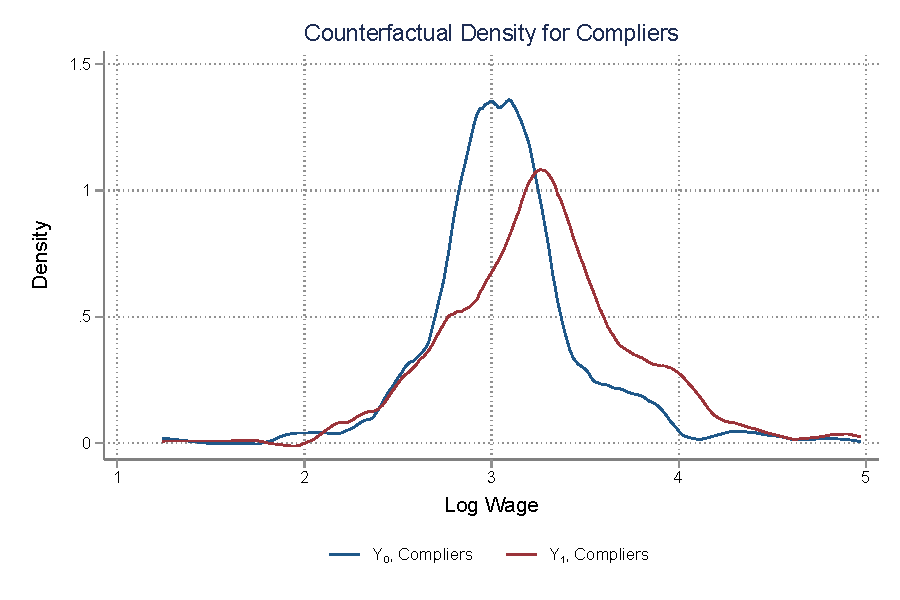
\includegraphics[width=0.8\textwidth]{ps3/figures/q4_partF_compliers.pdf}
\end{figure}
\end{solution}

\begin{problem}{g}
What can you say about $Y_{0}$ and $Y_{1}$ for always-takers and never-takers?
\end{problem}
\begin{solution}
Note that now the outcomes we are interested are observed in the data To calculate the mean of the outcome for always- and never-takers, we can just average over what is observed in the data. The means are reported in the table below:
\begin{table}[H]
    \centering
    \begin{tabular}{l*{1}{c}}
\hline\hline
            &        Mean\\
\hline
$ Y_0 $ for never-takers&       3.114\\
$ Y_1 $ for always-takers&       3.009\\
\hline\hline
\end{tabular}

    \caption{Mean of $Y_0$ for never-takers and $Y_1$ for always-takers}
\end{table}
And the distributions are plotted below:
\begin{figure}[H]
    \centering
    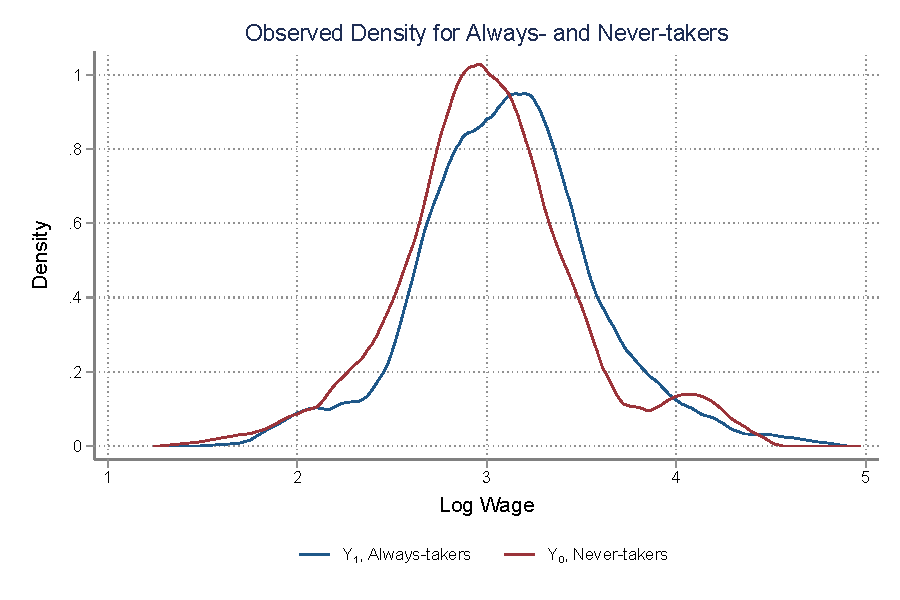
\includegraphics[width=0.8\textwidth]{ps3/figures/q4_partG_observed.pdf}
\end{figure}
\vspace{-1cm}
It is interesting that the distributions look quite similar. Those who go to medical school after losing the lottery have a distribution of wages in 2007 that are quite similar to those who don't go even if they are offered. Perhaps the never-takers know something about themselves and know that going to medical school won't increase their earnings, so that's why they'd never go and that explains the lack of a gap in the distributions.
\end{solution}

\begin{problem}{h}
The lottery is within lottery category and year, so your instrument is only exogenous within these groups. Estimate lottery category $\times$ year specific LATEs and combine these in one estimate. Compare this to the specification where you control for lottery category $\times$ year dummies and also interact the instrument with these dummies. Comment on your results.
\end{problem}
\begin{solution}
I follow Slide 59 of week3.pdf, which is based on Angrist \& Imbens (1995). I calculate the $x$-specific LATEs and the $x$-specific weights. The most important part of this procedure is to recognize that the expectations are over the density of $X$:
\begin{align*}
    \omega(x) &= \frac{\pi_x^2 \sigma_Z(x)}{E[\pi_x^2 \sigma_Z(x)]} = \frac{\pi_x^2 \sigma_Z(x)}{\sum_x \pi_x^2 \sigma_Z(x) P(X=x)} \\
    \beta &= E[\beta(x)\omega(x)] = \sum_x \beta(x)\omega(x) P(X=x)
\end{align*}

In the table below, proportion is $P(X=x)$ and weight is $\omega(x)$. For each row, we multiply these three together and then sum them to get $0.19156$, as is reported in the footnote.
\begin{table}[H]
    \centering
    \begin{center}
\begin{tabular}{ccccc}
\hline \noalign{\smallskip}Year & Lottery Category & $\beta(x)$ & Proportion & Weight\\
\noalign{\smallskip}\hline \noalign{\smallskip}1988 & 3 & -0.80 & 0.06 & 0.05\\
1988 & 4 & 0.12 & 0.14 & 0.37\\
1988 & 5 & 0.16 & 0.13 & 1.53\\
1988 & 6 & 0.21 & 0.18 & 1.89\\
1989 & 3 & 1.56 & 0.05 & 0.10\\
1989 & 4 & 0.01 & 0.13 & 0.21\\
1989 & 5 & 0.52 & 0.14 & 0.41\\
1989 & 6 & 0.15 & 0.17 & 1.89\\
\noalign{\smallskip}\hline\end{tabular}\\
\begin{footnotesize}$\beta=E[\beta(x)\omega(x)]$ is calculated as 0.19156\end{footnotesize}\\
\smallskip
\end{center}

\end{table}
The above specification compares favorably to the one where we control for lottery category $\times$ year dummies and also interact the instrument with these dummies. The coefficient below, $0.19152$, is only slightly off from the weighted-average version. This makes perfect sense, as the difference is probably due to estimation error and in a larger sample would become even smaller.
\begin{table}[H]
    \centering
    \begin{tabular}{l*{1}{c}}
\hline\hline
                    &\multicolumn{1}{c}{Log Wage}\\
\hline
Attended medical school&     0.19152\\
                    &   (0.05083)\\
[1em]
Lottery category=4 $\times$ Year=1989&    -0.00253\\
                    &   (0.06069)\\
[1em]
Lottery category=5 $\times$ Year=1989&     0.03112\\
                    &   (0.06002)\\
[1em]
Lottery category=6 $\times$ Year=1989&     0.01493\\
                    &   (0.06006)\\
[1em]
Constant            &     2.94840\\
                    &   (0.06917)\\
\hline
Observations        &        1476\\
\hline\hline
\multicolumn{2}{l}{\footnotesize Standard errors in parentheses}\\
\end{tabular}

\end{table}
The results show that the causal impact of attending medical school on wages is positive and that doing so leads to wages that are $\operatorname{exp}(.19152)-1=21\%$ higher than not attending medical school. This certainly seems plausible, since medical school training is intensive and can lead to large gains in human capital.
    




\end{solution}

\end{document}
